\documentclass{article}
\usepackage{graphicx}
\usepackage{amsmath}
\usepackage{listings}
\title{Implementing the exponential function in C}
\author{T.T.~Lindkvist}
\date{}
\begin{document}
    \maketitle
    \section{Making the computer understand}
    As we know the exponential function \texttt{exp(x)}, is simply Euler's number, $e\approx2.71828$, raised to the power of $x$ - \texttt{exp(x)} $=e^x$. However, computers really only know the simple operators +, -, * and /. Using the Taylor series for the exponential function, we can easily implement it
    \begin{align}
        e^x = \sum_{n=0}^{\infty} \frac{x^n}{n!} = 1 + x + \frac{x^2}{2} + \frac{x^3}{6} + \cdots
    \end{align}
	Of course we cannot do an infinite sum, but luckily this converges fast for small x. So we take the first $N=10$ terms. This leaves a problem for larger $x$'s, where the approximation is not so good. To combat this, we can use a rule of exponents
	\begin{align}
		e^x = e^{x/2}\cdot e^{x/2} \;.
	\end{align}
	Suppose we want to compute \texttt{exp(x)} for some $x$ larger than some $x_{max}$, where we know precision becomes an issue, we simply apply this rule of exponents recursively until we can get by, by calculating \texttt{exp(x')} for some $x'=x/2^n<x_{max}$.
	We can also make use of another property of exponents
	\begin{align}
		e^{-x} = \frac{1}{e^x} \;,
	\end{align}
	and hereby only need to evaluate the function for positive argument $x$ - making all terms in the series positive. We do this, since summing terms of alternating sign can make the calculation lose precision, since the terms are of comparable order of magnitude. Also, in order to not lose precision when adding the smaller (higher order, since $ x $ is small) terms, one could add the numbers from highest to lowest order, or in order to not use so many multiplications, write the terms inside one another, in this convoluted fashion.
	\begin{align*}
		\sum_{n=0}^{N} \frac{x^n}{n!} = 
		1+x\left(1+\frac{x}{2}\left(1+\frac{x}{3}\left(1+\frac{x}{4}\left(1+\frac{x}{5}\left(1+\frac{x}{6}\left(\cdots\right)\right)\right)\right)\right)\right)
	\end{align*}
\section{C Implementation}
Suppose we choose the maximum $ x $, where the Taylor expansion is directly used, $ x_{max} = 1/8 $, and a maximum order of evaluation $ N=10 $, then the function can be written in C, like this:
\lstset{language=Pascal}
\begin{lstlisting}
double ex(double x){
    if(x<0)    return 1/ex(-x);
    if(x>1./8) return pow(ex(x/2), 2);
    return 1+x*(1+x/2*(1+x/3*(1+x/4*(1+x/5*\
    (1+x/6*(1+x/7*(1+x/8*(1+x/9*(1+x/10)))))))));
}
\end{lstlisting}
\section{Comparison of implementations}
On figure \ref{fig:1}, our implementation is plotted together with the implementation from \texttt{math.h}. As seen, they give approximately the same values, and with a very low relative error $<10^{-14}$, as seen on figure \ref{fig:relative}.
\begin{figure}[h]
	\centering
	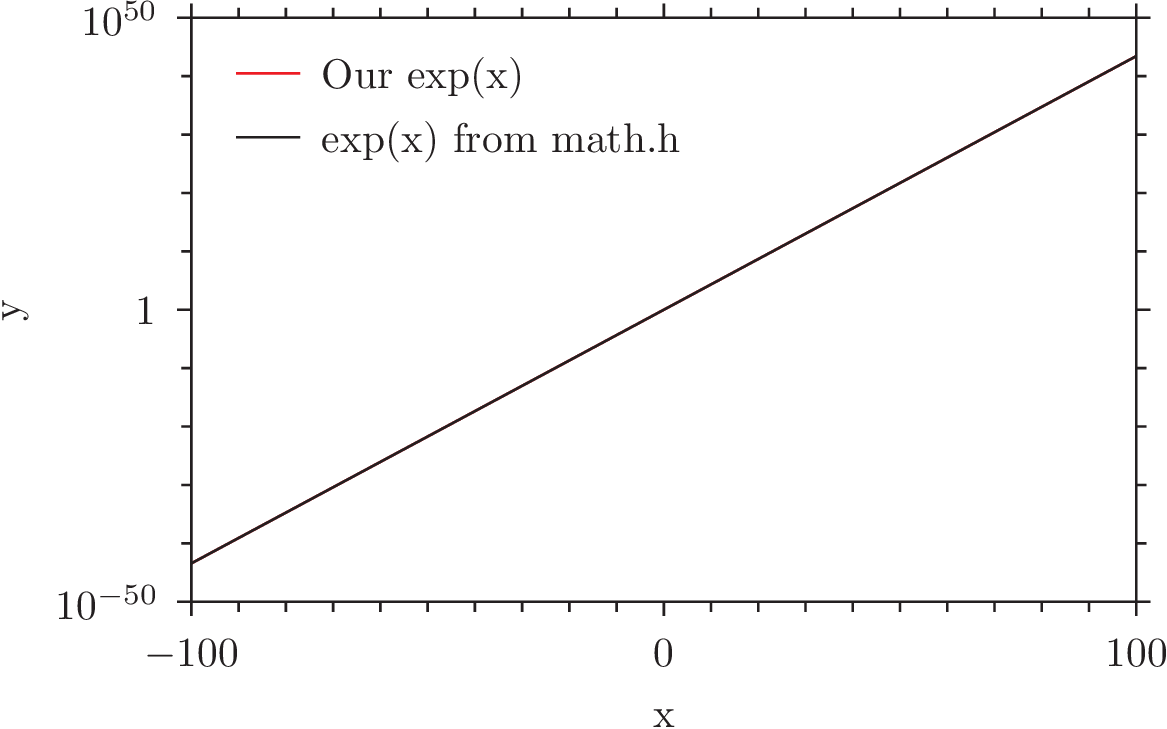
\includegraphics{plot1.png}
	\caption{Shows our implementation together with the implementation from \texttt{math.h}. Note: the y-axis is logarithmic.}
	\label{fig:1}
\end{figure}
\begin{figure}[h]
	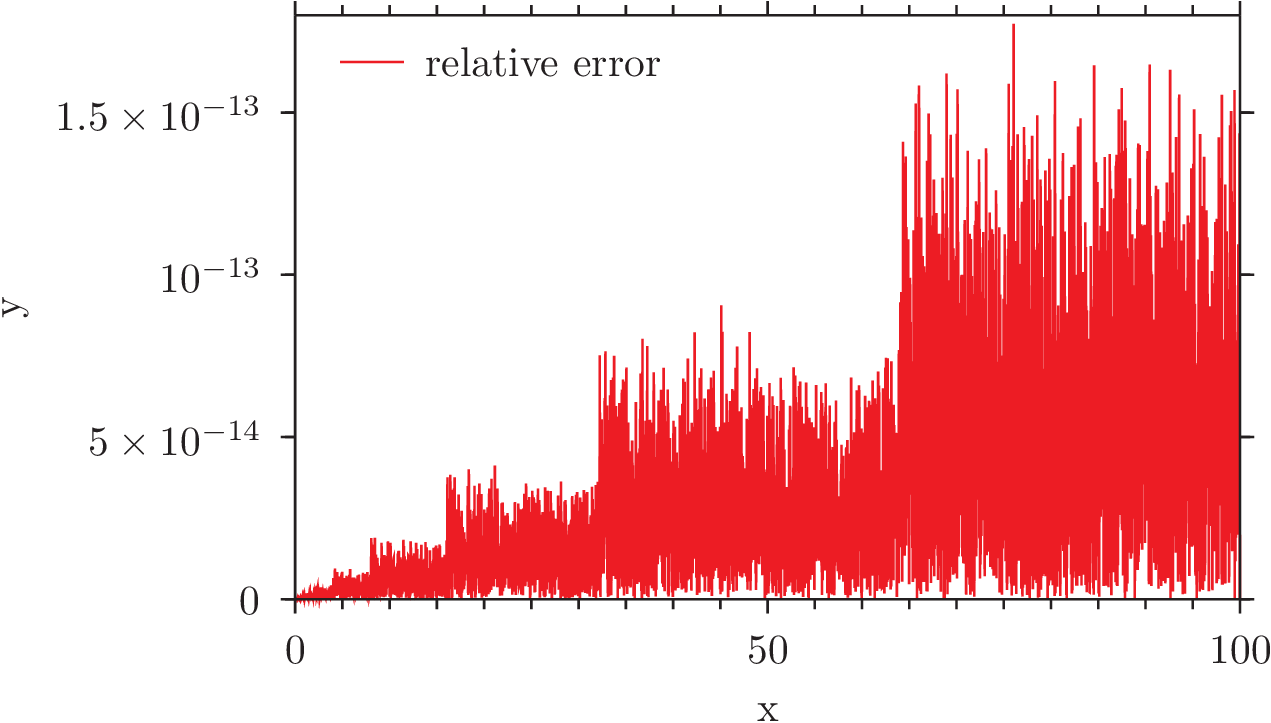
\includegraphics{plot2.png}
	\caption{Shows the relative error of our implementation compared to the \textit{correct} implementation from \texttt{math.h}. Note: the y-axis is logarithmic.}
	\label{fig:relative}
\end{figure}
We can also look at the difference between only calculating the positive terms, and also evaluating the Taylor series with negative terms. On figure \ref{fig:negative} the relative error of the two expressions, with respect to \texttt{exp} from \texttt{math.h}. These expressions are of course equal for positive $ x $, but at negative $ x $, the expression with the negative terms, is actually more precise.
\begin{figure}[h]
	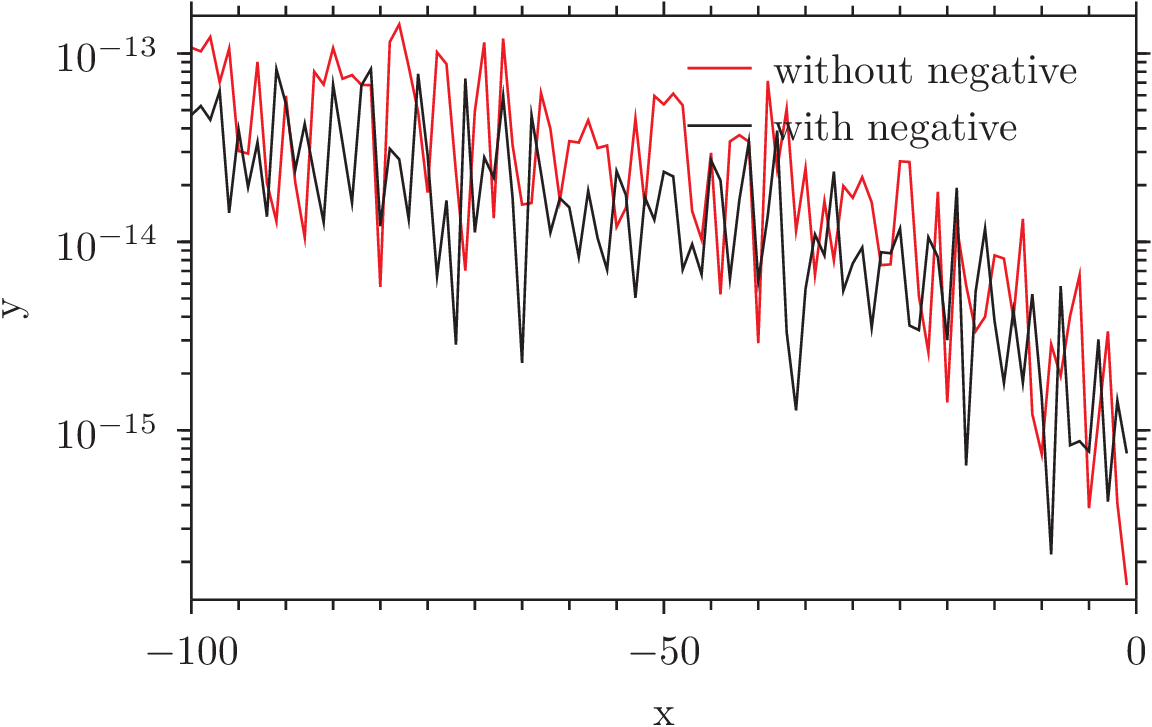
\includegraphics{plot3.png}
	\caption{Shows the relative error of our implementation with and without evaluation of negative terms.}
	\label{fig:negative}
\end{figure}
We can also take a look at using the convoluted expression versus the ordinary sum of terms. This can be seen on figure \ref{fig:summation}. Since we are using doubles, this yielded no difference when summing backwards from highest to lowest order, but when evaluating from lowest to highest order, a difference occurred, and this is slightly more imprecise.
\begin{figure}[h]
	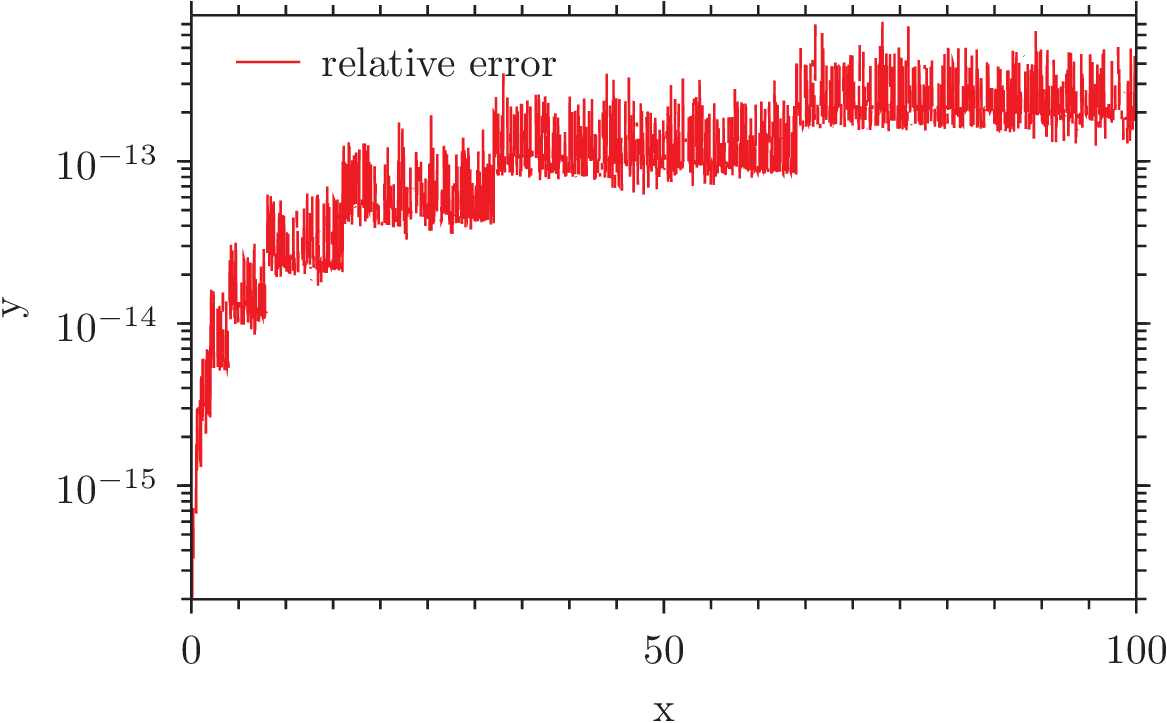
\includegraphics{plot4.png}
	\caption{Shows the relative error of the convoluted expression and summing the terms from lowest to highest order.}
	\label{fig:summation}
\end{figure}

Small note: steps can be seen on the graphs at powers of two - since the cutoff from direct evaluation of the Taylor series is a power of two. This is better seen with a large number of evaluation points, so this is better illustrated on figure \ref{fig:largeN}.
\begin{figure}[h]
	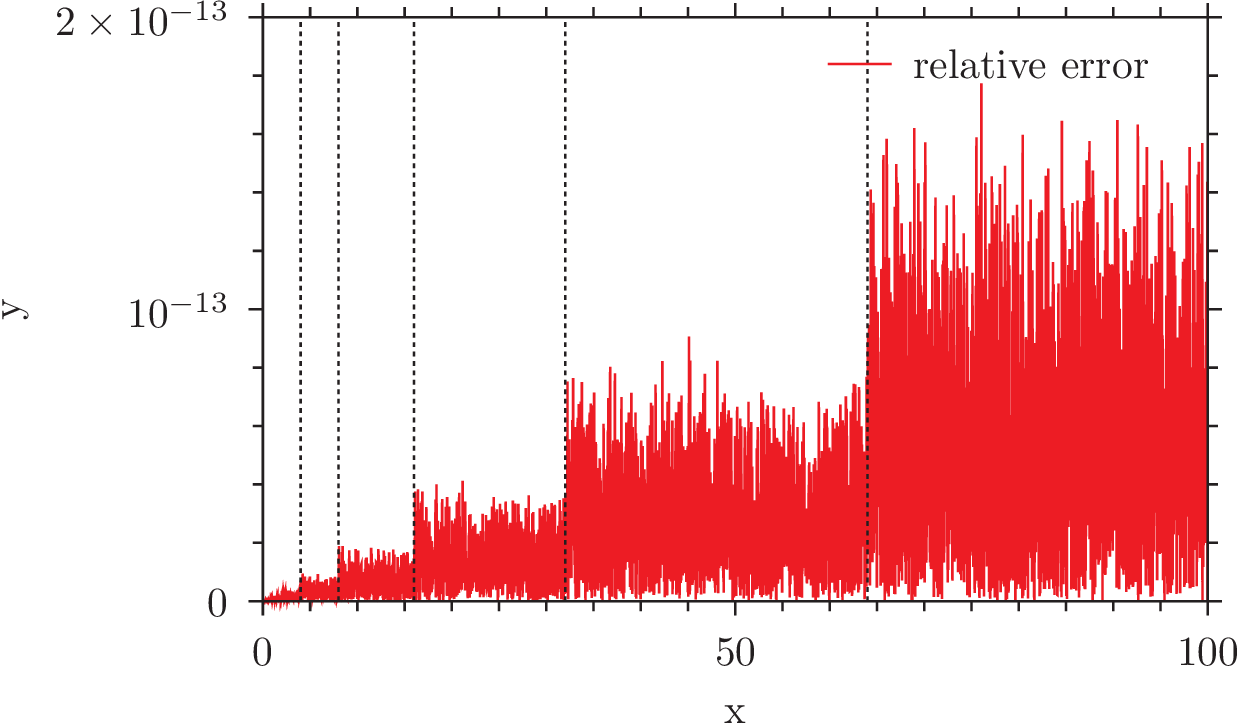
\includegraphics{plot5.png}
	\caption{Replica of figure \ref{fig:relative}, but with larger number of evaluation points and with dashed lines for multiples of two ($2^n$ for $ n>1 $)}
	\label{fig:largeN}
\end{figure}
\end{document}	